\section{System And Controller}

The system has three explicit knowledge substrates:
\begin{itemize}[leftmargin=1.5em]
\item frozen parametric knowledge from the base model,
\item persistent external memory,
\item a detachable patch bank for temporary and durable updates.
\end{itemize}

The controller is a LinUCB-style contextual bandit with a separate learned future-value regressor. For each valid action $a$, it scores
\[
\mathrm{score}_t(a) = x_t^\top \theta_a + \alpha \sqrt{x_t^\top A_a^{-1} x_t} + \mathrm{prior}_a(x_t) + \lambda_e \hat V_a(x_t),
\]
where $x_t$ is the full \texttt{RouterFeatures} vector, $\alpha = 0.6$, $A_a$ is initialized to the identity matrix, $b_a$ is initialized to zero, and $\theta_a = A_a^{-1} b_a$. The coefficient $\lambda_e$ is 1.0 for the base router, 0 when delayed utility is disabled, and the public-track calibration scale for \texttt{router\_calibrated}. The fixed action prior $\mathrm{prior}_a(x_t)$ is action-specific and implementation-defined: it favors confident parametric answers for \texttt{PARAM\_ONLY}, aligned/high-hit states for \texttt{READ\_MEMORY}, high retrieval quality for \texttt{RETRIEVE}, and stable recurrent regimes for write, adapt, and consolidate actions. After each routed episode, the chosen arm is updated online by $A_a \leftarrow A_a + x_t x_t^\top$ and $b_a \leftarrow b_a + r_t x_t$.

\paragraph{Feature provenance.}
The runtime-derived features are the current model confidence, the quality of the top retrieved document, the memory-hit score, the memory-alignment score, the time since the last memory update, and whether the immediately preceding action was a retrieval. The benchmark-provided or metadata-derived features are recurrence, stability, volatility, contradiction risk, source-agreement count, domain-change rate, popularity bin, question-seen status, answer-changed status, weeks since the last change, alias availability, and prior stale-answer availability. The implementation also includes a derived forgetting-risk feature, computed as $\max(0, \text{volatility} + 0.2 \cdot \text{update\_expected})$, so that public correction chains and propagation-heavy edits pay a larger mutation penalty than stable recurrence.

\paragraph{Future-value estimator.}
Delayed utility is learned by a separate linear regressor for each action. The future-value basis contains five features: recurrence, stability, source-agreement count, volatility, and contradiction risk. Each action starts from a small heuristic weight vector that reflects its intended reuse pattern, and those weights are updated online with learning rate 0.05. The target is the observed future utility over the next three episodes. That utility credits repeated subject/relation reuse and domain updates; on the public track it gives nonzero credit to write/adapt actions only when the question has been seen before and answer-change or stale-answer evidence is already present, and it requires at least two confirmations before consolidation receives delayed-utility credit.

\paragraph{Public-track calibration.}
The calibrated controller does not change the action inventory or the immediate bandit term. It only rescales delayed utility through \texttt{calibrated\_future\_value\_scale}. The scale depends on whether the question was seen before, whether the answer changed since the previous appearance, whether a stale prior answer is available, the update type, confirmation and change counts, recurrence, volatility, contradiction risk, retrieval quality, alias availability, and stability/volatility classes. Stable confirmations can restore the scale up to 0.9, while safe forgetting probes can restore it up to 0.55; unstable public cases can push the scale close to zero.

\paragraph{Execution semantics.}
Retrieval uses BM25 over the benchmark-provided support documents or cached local corpora. The controller uses top-$k=3$ retrieval by default and top-$k=5$ on freshness/adaptation/consolidation paths; freshness-style tasks also enforce a timestamp filter so only evidence available at the current episode time can be used. On freshness/public benchmarks, the answer is selected directly from the retrieved support documents: \texttt{retrieve} uses the highest trust-plus-relevance document, while \texttt{adapt} uses the latest/high-trust document. On PopQA, MQuAKE, and UniEdit, the retrieved documents are passed to the underlying QA model through an evidence-conditioned prompt. Memory queries return the highest-support, highest-stability, latest record for the current subject--relation pair. \texttt{PARAM\_ONLY} first checks active temporary or durable patches, then falls back to the base model. \texttt{FAST\_ADAPT} creates a temporary patch whose horizon comes from benchmark metadata. \texttt{CONSOLIDATE} promotes the current temporary patch, creating one on demand if a confirmation episode qualifies. Rollback removes a durable patch when a rollback probe retrieves evidence that disagrees with the promoted answer.

\paragraph{Write and consolidation guards.}
Memory writes and consolidations are controlled by deterministic masks rather than by free-form generation. The base write gate requires sufficient retrieval quality, nontrivial recurrence, at least one supporting source, and no existing memory record; the PopQA guardrails then tighten those thresholds further so weak-recurrence cases default back to retrieval. On freshness-style tasks, volatile or corrective updates disable memory writes; on the public track, writes are re-enabled only for answer-changing or stale-answer cases, or for unseen but unusually stable high-confidence cases. Consolidation requires at least two supporting sources, recurrence at least 0.6, stability at least 0.7, volatility at most 0.3, contradiction risk at most 0.3, and no recent rollback. The public track adds stronger conditions: the question must have been seen before, the answer must already have changed, at least one earlier change and two confirmations must be present, and the current episode must be a stable confirmation.

\begin{table}[h]
\centering
\small
\begin{tabular}{p{0.97\linewidth}}
\toprule
\textbf{1. Build features.} Compute the full feature vector $x_t$ from the current episode, world state, retrieval evidence, memory state, change-tracking metadata, and recent action history. \\
\textbf{2. Compute regime masks.} Apply the benchmark-specific guardrails and mark each action in $\mathcal{A}$ as valid or invalid. \\
\textbf{3. Score valid actions.} For each valid action $a$, compute $x_t^\top \theta_a + \alpha \sqrt{x_t^\top A_a^{-1} x_t} + \mathrm{prior}_a(x_t) + \lambda_e \hat V_a(x_t)$. \\
\textbf{4. Select action.} Choose $a_t = \arg\max_{a \in \mathcal{A}_{\mathrm{valid}}} \mathrm{score}_t(a)$. \\
\textbf{5. Execute action.} Run the corresponding parametric, retrieval, memory, or patch operation and collect the answer, evidence ids, touched state, and side effects. \\
\textbf{6. Compute reward.} Evaluate answer quality, latency and operation cost, forgetting penalty, and delayed utility to obtain $r_t$. \\
\textbf{7. Update estimators.} Set $A_{a_t} \leftarrow A_{a_t} + x_t x_t^\top$, $b_{a_t} \leftarrow b_{a_t} + r_t x_t$, recompute $\theta_{a_t}$, and update the action-specific future-value regressor with the observed next-three-episode utility. \\
\textbf{8. Log trace.} Store the action mask, action scores, feature vector, reward breakdown, evidence ids, state mutations, and benchmark metrics for later aggregation. \\
\bottomrule
\end{tabular}

\caption{Algorithm 1. Multi-timescale routing policy. The policy scores six actions with one utility objective, applies benchmark-aware masks, executes the chosen operation, and logs the resulting state changes.}
\label{tab:router-algorithm}
\end{table}

\begin{figure}[h]
\centering
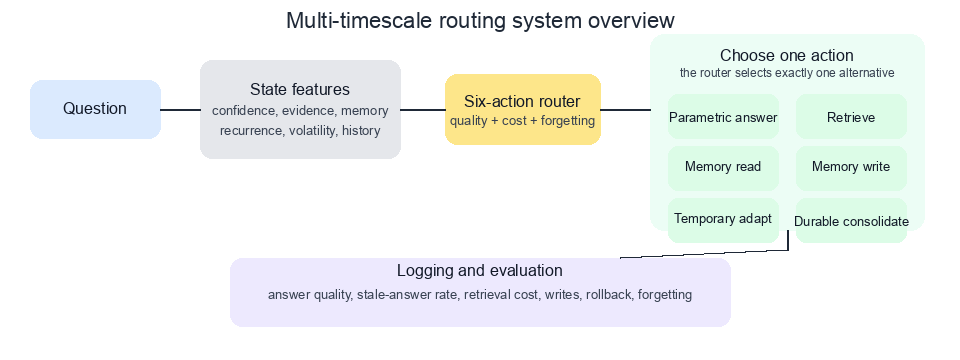
\includegraphics[width=0.95\linewidth]{../shared/generated/word_assets/fig_system_overview.png}
\caption{System overview. A question and its state features are routed to one of six actions: parametric answering, retrieval, memory read, memory write, temporary adaptation, or durable consolidation. Every episode records action usage, answer quality, stale-answer behavior, rollback, and forgetting-related metrics.}
\label{fig:system-overview}
\end{figure}

\paragraph{Temporary adaptation.}
The implementation keeps \texttt{FAST\_ADAPT} lightweight: it attaches a temporary patch with a bounded horizon rather than training a full adapter. This choice keeps the controller claim separate from the heavier engineering trade-offs explored in dedicated editing systems such as MELO and WISE \citep{yu2023melo,wang2024wise}.

\paragraph{Durable consolidation.}
\texttt{CONSOLIDATE} promotes a validated temporary patch into the durable patch bank. This path is rare by design, requires the guard conditions above, and is blocked after rollback.

\paragraph{Rollback.}
Correction episodes can invalidate a previously durable answer. The implementation explicitly records whether rollback was triggered, whether a durable patch was used, and whether forgetting probes remain correct afterward.
